\documentclass[12pt]{article}
\usepackage{url,graphicx,tabularx,array,geometry,enumitem,amsmath}
\setlength{\parskip}{1ex} %--skip lines between paragraphs
\setlength{\parindent}{0pt} %--don't indent paragraphs

%-- Commands for header
\renewcommand{\title}[1]{\textbf{#1}\\}
\renewcommand{\line}{\begin{tabularx}{\textwidth}{X>{\raggedleft}X}\hline\\\end{tabularx}\\[-0.5cm]}
\newcommand{\leftright}[2]{\begin{tabularx}{\textwidth}{X>{\raggedleft}X}#1%
& #2\\\end{tabularx}\\[-0.5cm]}

%\linespread{2} %-- Uncomment for Double Space
\begin{document}

\title{Digital Signal Processing - Assignment 4}
\line
\leftright{\today}{Stephanie Lund (2555914)\\Aljoscha Dietrich(2557976)} %-- left and right positions in the header

\section*{Exercise 1}

\subsection*{1.1}
The LPC technique predicts the next values from a given signal. It is based on the source-filter model of speech production, which states that speech is created by a source (the vocal cords) and an independent filter (the vocal tract) which creates resonances (formants). It is useful for encoding compressed speech.

\subsection*{1.2}
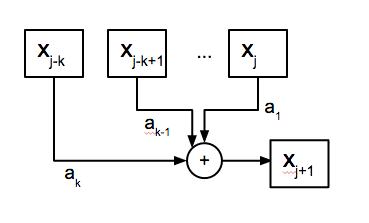
\includegraphics[scale=0.65]{hw4-2.png}
\begin{align*}
	x_{j+1} = \sum_{i=0}^{k} a_i x_{j-i}
\end{align*}

\subsection*{1.3}
The error equation for some measured $x_n$ is: $e_n = x_n + \sum_{i=1}^k a_i x_{n-i}$\\\\
We want to minimize the squared error $\mathcal{E} = E[ |e^2| ]$ with respect to the $a_k$ parameters.\\\\
Therefore, we want to minimize $\mathcal{E} = \frac{1}{N} \sum_{n=1}^N (x_n + \sum_{k=1}^p a_k x_{n-k})^2$\\\\
We can do this by taking the derivative to get $\mathcal{E} = - \frac{1}{N} \sum_{n=1}^N x_n x_{n-k}$.

\subsection*{1.4}
We start with:
\begin{align*}
x(n) &= [-2, 0, 1, -1, 0, 2]\\
x(n+1) &= [0, 1, -1, 0, 2, 0]\\
x(n+2) &= [1, -1, 0, 2, 0, 0]\\
\end{align*}

Therefore, the autocorrelation matrix $R_{xx}$ with order 2 and window size of 6 is:
\begin{align*}
\begin{bmatrix}
x(n)*x(n) & x(n)*x(n+1) \\
x(n)*x(n+1) & x(n)*x(n)
\end{bmatrix}
= \begin{bmatrix}
10/6 & -1/6 \\
-1/6 & 10/6
\end{bmatrix}
\end{align*}

We want to solve for:

\begin{align*}
R_{xx}
\begin{bmatrix}
a_1 \\
a_2
\end{bmatrix}
=
\begin{bmatrix}
x(n) * x(n+1) \\
x(n+1) * x(n+2)
\end{bmatrix}
=
\begin{bmatrix}
-1/6 \\
-4/6
\end{bmatrix}
\end{align*}

Solving this system, we get:

\begin{align*}
a_1 = -\frac{14}{99} \qquad a_2 = -\frac{41}{99}
\end{align*}

Therefore we have the prediction:
\begin{align*}
f[6] = a_1 * f[5] + a_2 * f[4] = -\frac{28}{99}
\end{align*}


\subsection*{1.5}
\begin{align*}
f[2] = a_1 * f[1] + a_2 * f[0] = &\frac{82}{99} \\
f[3] = -&\frac{14}{99} \\
f[4] = -&\frac{27}{99} \\
f[5] = &\frac{41}{99}
\end{align*}

The errors are:\\
\begin{align*}
e_2 =  &\frac{17}{99}\\
e_3 = &-\frac{85}{99}\\
e_4 =&  \frac{27}{99}\\
e_5 =& \frac{157}{99}\\
\end{align*}

\subsection*{1.6}
TODO

\end{document}